\documentclass[tikz,border=10pt,multi=tikzpicture]{standalone}
\usepackage{xcolor}
\usetikzlibrary{calc}
\definecolor{mainblue}{HTML}{001158}
\definecolor{accent}{HTML}{8592bc}
\definecolor{lightaccent}{HTML}{e7e9f2}
\definecolor{loadcolor}{HTML}{e67e22}
\definecolor{defcolor}{HTML}{c1121f}

\begin{document}

% ===== PAGE 1: wind turbine - tower clearance =====
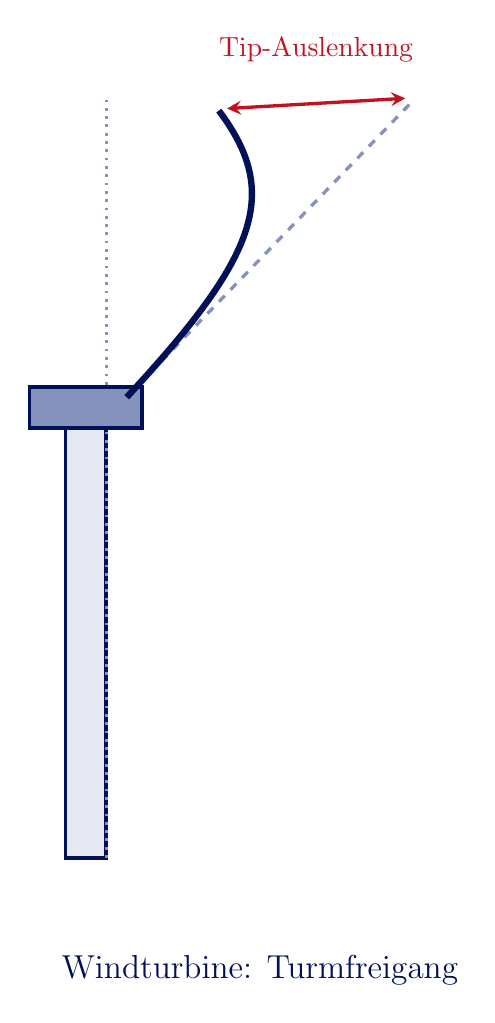
\begin{tikzpicture}[>=stealth, font=\Large, scale=1.3]
  \fill[lightaccent] (-0.2,0) rectangle (0.2,4.2);
  \draw[mainblue, line width=1.3pt] (-0.2,0) rectangle (0.2,4.2);
  \fill[accent] (-0.55,4.2) rectangle (0.55,4.6);
  \draw[mainblue, line width=1.3pt] (-0.55,4.2) rectangle (0.55,4.6);

  \draw[accent, dashed, line width=1.2pt] (0.4,4.5) -- (3.2,7.4);
  \draw[mainblue, line width=2.3pt] (0.4,4.5) .. controls (1.7,5.9) and (1.9,6.5) .. (1.3,7.3);
  \draw[defcolor, <->, line width=1.2pt] (1.38,7.32) -- (3.12,7.42);
  \node[defcolor, font=\normalsize] at (2.25,7.9) {Tip-Auslenkung};

  \draw[accent, dotted, line width=1pt] (0.2,0) -- (0.2,7.4);
  \node[mainblue, align=center, font=\large] at (1.7,-1.1) {Windturbine: Turmfreigang};
\end{tikzpicture}

% ===== PAGE 2: aircraft wing - U-2 style, needs tip support wheel =====
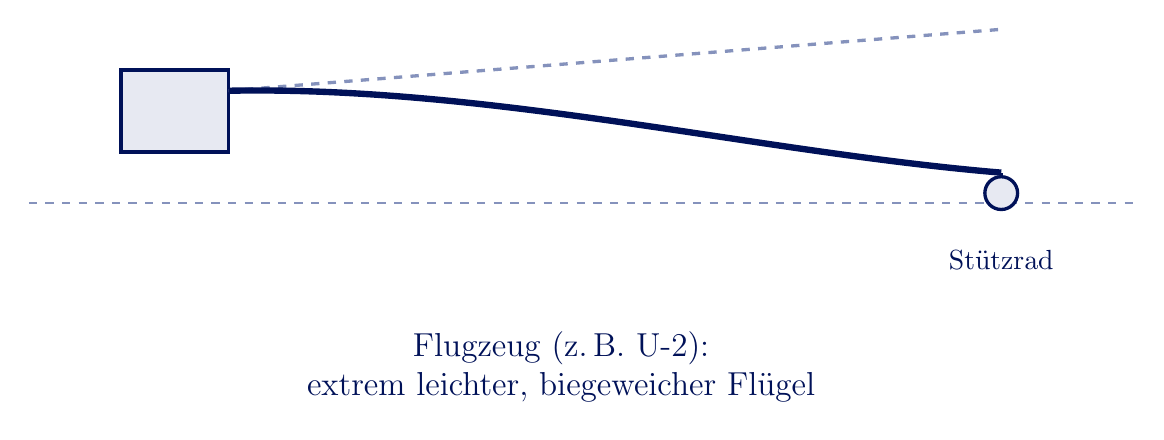
\begin{tikzpicture}[>=stealth, font=\Large, scale=1.3]
  \draw[accent, dashed, line width=0.8pt] (-1.3,0) -- (9.5,0);
  \fill[lightaccent] (-0.4,0.5) rectangle (0.65,1.3);
  \draw[mainblue, line width=1.3pt] (-0.4,0.5) rectangle (0.65,1.3);

  \draw[accent, dashed, line width=1.2pt] (0.65,1.1) -- (8.2,1.7);
  \draw[mainblue, line width=2.3pt] (0.65,1.1) .. controls (3.2,1.15) and (5.8,0.5) .. (8.2,0.3);

  \draw[mainblue, line width=1.2pt, fill=lightaccent] (8.2,0.1) circle (0.16);
  \draw[mainblue, line width=1pt] (8.2,0.26) -- (8.2,0.3);
  \node[mainblue, align=center, font=\normalsize] at (8.2,-0.55) {St\"utzrad};

  \node[mainblue, align=center, font=\large] at (3.9,-1.6) {Flugzeug (z.\,B.\ U-2):\\extrem leichter, biegeweicher Fl\"ugel};
\end{tikzpicture}

% ===== PAGE 3: leaf spring - low stiffness is the function =====
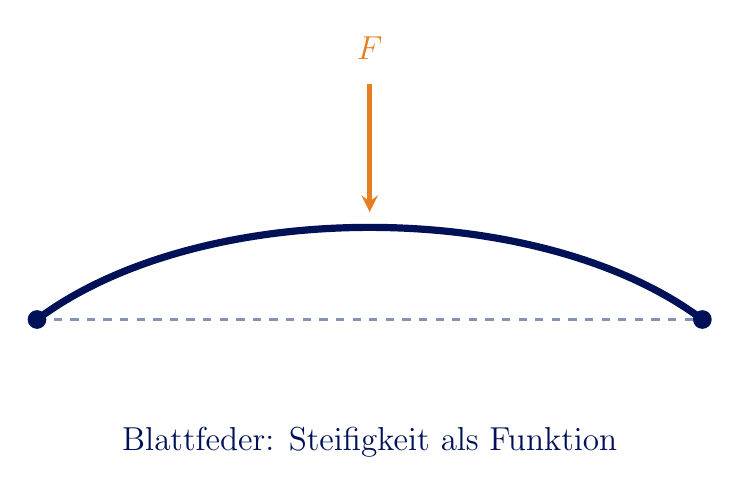
\begin{tikzpicture}[>=stealth, font=\Large, scale=1.3]
  \draw[accent, dashed, line width=1.2pt] (0,0) -- (6.5,0);
  \draw[mainblue, line width=2.6pt] (0,0) .. controls (1.6,1.2) and (4.9,1.2) .. (6.5,0);
  \draw[loadcolor, ->, line width=1.6pt] (3.25,2.3) -- (3.25,1.05);
  \node[loadcolor, font=\large] at (3.25,2.65) {$F$};
  \fill[mainblue] (0,0) circle (2.6pt);
  \fill[mainblue] (6.5,0) circle (2.6pt);
  \node[mainblue, align=center, font=\large] at (3.25,-1.2) {Blattfeder: Steifigkeit als Funktion};
\end{tikzpicture}

\end{document}
